\chapter{Una breve introducci�n a la norma IEC 61850 aplicada a centrales hidroel�ctricas
y a los aspectos t�cnicos de un regulador de velocidad t�pico de Itaipu}
%\chapter{Una breve introducci�n a la norma IEC 61850 y su aplicaci�n a
%centrales hidroel�ctricas}
\label{ch:introduction}

\section{IEC 61850: Una norma para todo el sistema de comunicaci�n del proceso
el�ctrico}

Para resolver los pr�ximos desaf�os del sector de la energ�a en todo el mundo,
se est� realizando un importante trabajo en la integraci�n de las tecnolog�as
de informaci�n y comunicaci�n digital a las tecnolog�as del sector el�ctrico
\cite{Kruimer:2003}. Este proceso tiene como caracter�stica principal la
consolidaci�n y adopci�n de nuevas normas t�cnicas internacionales, entre las
cuales la IEC 61850 cumple un papel fundamental. Uno de los requisitos m�s
importantes en el dise�o de los modernos 
sistemas el�ctricos de potencia es la interoperabilidad
sint�ctica y sem�ntica entre los equipamientos de automatizaci�n y control
utilizados. Esto s�lo puede ser alcanzado estableciendo protocolos comunes,
basados en normas. La interoperabilidad sem�ntica referida anteriormente
establece una congruencia en t�rminos y significado de la informaci�n del
sistema, mientras que la interoperabilidad sint�ctica permite la codificaci�n,
decodificaci�n, el transporte y el direccionamiento preciso de la informaci�n
intercambiada entre los equipamientos a trav�s de la red de comunicaci�n del
sistema el�ctrico.             

La norma IEC 61850, desarrollada en conjunto por m�s de 60 expertos de Am�rica
y Europa, es la primera norma adoptada a nivel global en el �rea de las
comunicaciones en subestaciones. Gran parte de la aceptaci�n de esta norma se
debe a que, adem�s de especificar la utilizaci�n y la combinaci�n adecuada de
una pila de protocolos de comunicaci�n ya existentes, provee una interfaz
dise�ada en forma abstracta, logrando as� el desarrollo de proyectos m�s
sofisticados y a prueba de futuro \cite{Mackiewicz:2006}. La norma IEC 61850
tambi�n define el proceso de ingenier�a a ser implementado en el dise�o del sistema de
automatizaci�n, las caracter�sticas b�sicas de las herramientas a utilizar para
dicho proceso, y los procedimientos precisos para la configuraci�n de los
aspectos de comunicaci�n de los dispositivos.          



%The IEC 61850 is a standard for communication networks and systems 
%and the related system requirements for the whole electrical system
%used by \Glspl{IED} to perform the required functions for the secundary
%equipments.


%\begin{figure}
%  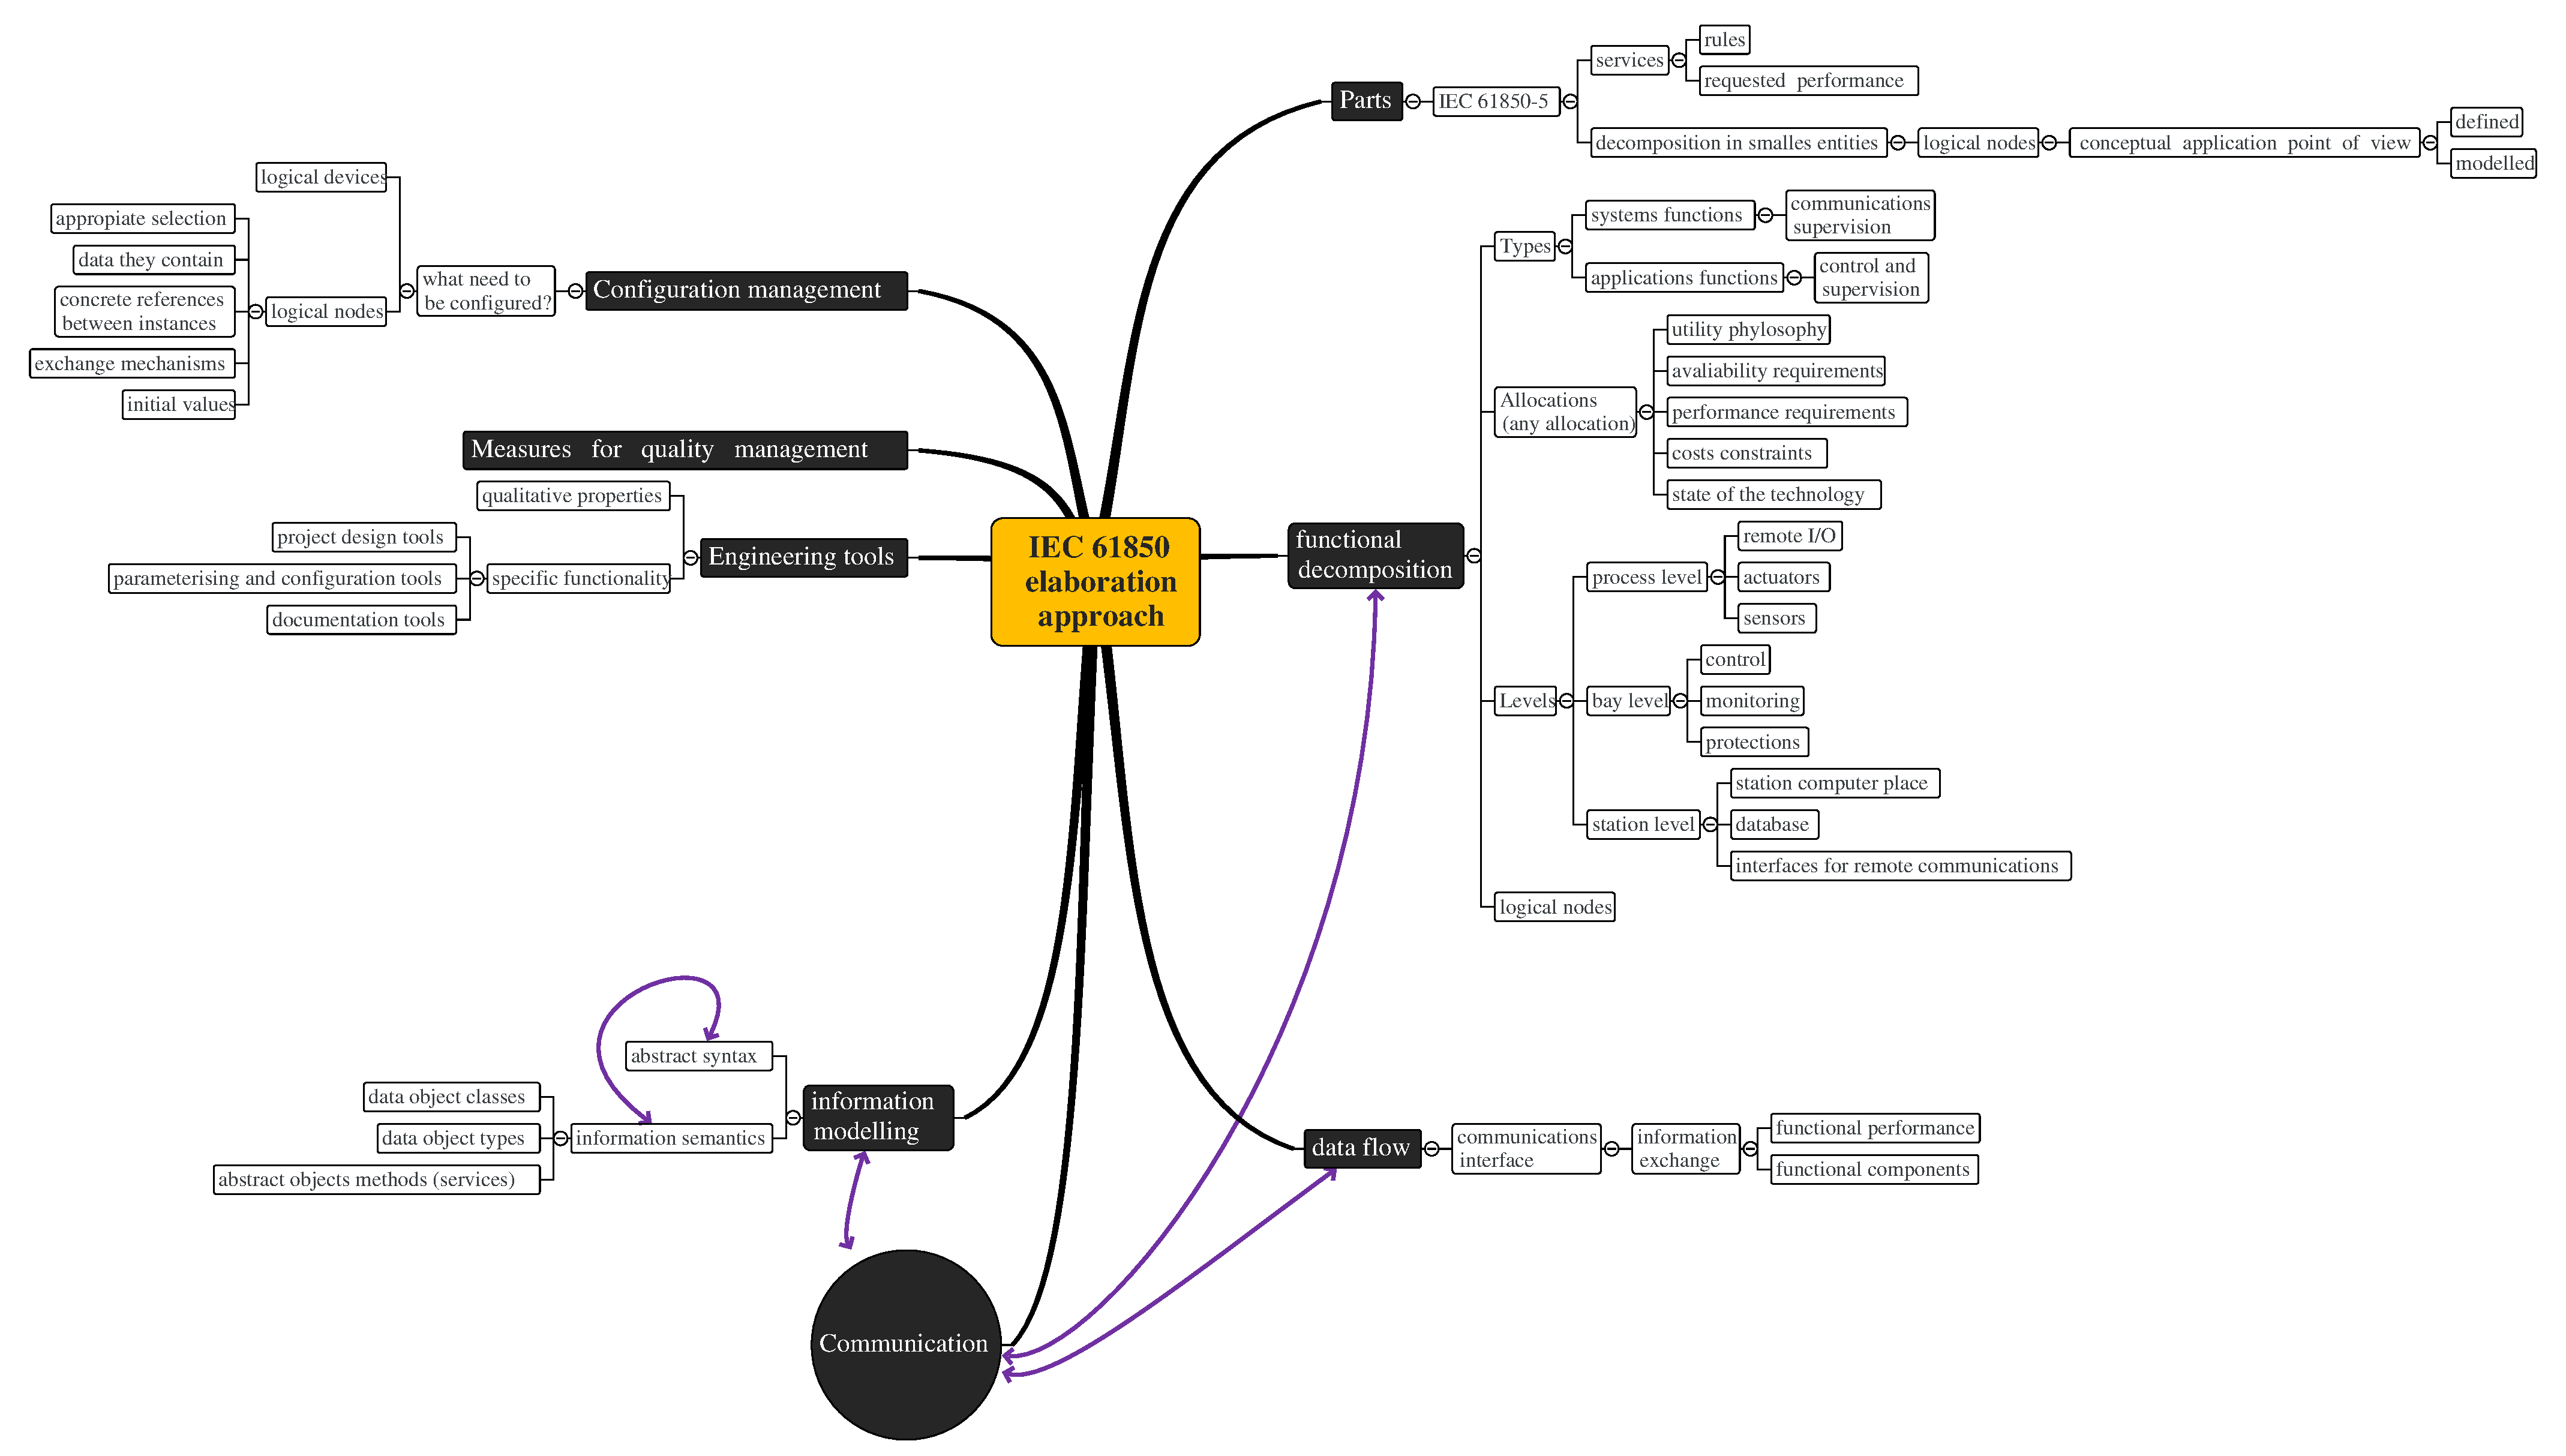
\includegraphics[width=1.0\textwidth]{appendices/IEC61850approach}
%  \caption{Borrador - Esquema del futuro capitulo }
%  \label{fig:lan-networks-topologies-fig3}
%\end{figure}


\section{Objetivos de la norma IEC 61850}

%El objetivo principal de la norma IEC 61850 es la normalizaci�n 
%de la comunicaci�n utilizada en la automatizaci�n de los 
%sistemas el�ctricos de potencia. 

 
El objetivo de la norma IEC 61850 es 
permitir la interoperabilidad entre IEDs
de diferentes fabricantes utilizados en la automatizaci�n de los 
sistemas el�ctricos del sistema el�ctrico. En este caso, 
la interoperabilidad se define como la habilidad de que 
los IEDs operen en la misma red de comunicaci�n compartiendo informaci�n y comandos,
respetando los requisitos funcionales y de desempe�o requeridos, y 
soportando futuros avances tecnol�gicos.

Este objetivo es alcanzado a trav�s de la descomposici�n 
de las interfaces de comunicaci�n en nodos l�gicos
dotados de sintaxis abstractas y sem�nticas 
de la informaci�n a ser intercambiada.
\section{Interoperabilidad}

El requisito m�s importante para la
construcci�n de los grandes sistemas el�ctricos  
acorde a las necesidades actuales es la interoperabilidad en el intercambio de
la informaci�n entre los dispositivos del sistema 
de automatizaci�n de subestaciones.

Gracias a la norma IEC 61850, dos o m�s \Glspl{IED}
del mismo fabricante, o de diferentes fabricantes, tienen
la habilidad de intercambiar informaci�n y utilizar dicha 
informaci�n para la ejecuci�n correcta de funciones espec�ficas
\cite{IEC61850-1:2003}.



\section{Tecnolog�as de comunicaci�n y redes}

La norma IEC 61850 est� dise�ada utilizando especificaciones y normas 
internacionales  de comunicaci�n basadas en Ethernet que permiten la
codificaci�n, decodificaci�n, el transporte y el direccionamiento preciso de la
informaci�n intercambiada entre los equipamientos a trav�s de la red de
comunicaci�n del sistema el�ctrico.      

La figura \ref{fig:pila-protocolos} presenta la pila de protocolos utilizada 
actualmente en la norma IEC 61850.


\begin{figure}
\begin{center}
  \includegraphics[width=1.0\textwidth]{chapters/introduction/figures/pila-de-protocolos.eps}
  \caption{Pila de protocolos utilizados en la norma IEC 61850}
  \label{fig:pila-protocolos}
\end{center}
\end{figure}

	
\section{Modelo de la informaci�n}
\label{sec:Modelo-informacion-61850}
La norma IEC 61850 define un modelo de informaci�n 
orientado a objetos, y organiza dicho modelo en 
tres niveles: nivel 1, nivel 2 y nivel 3. Este modelo
de informaci�n provee una estructura normalizada
de datos que cubre las necesidades del 
sistema el�ctrico \cite{Ozansoy:2009}. En las figuras
\ref{fig:Intro-LNs} y 
\ref{fig:virtualizacion-LNs} 
se presentan  
el modelo de informaci�n existente en sistemas
de potencia reales, sus equipamientos, 
y la representaci�n virtual del sistema el�ctrico
a trav�s del modelo IEC 61850 que 
responde con el mismo comportamiento que
en el mundo real, pero ejecut�ndose por software.

%\begin{landscape}
\begin{figure}
\begin{center}
  \includegraphics[width=1.0\linewidth]{chapters/introduction/figures/nodos-logicos.eps}
  \caption{Nodos l�gicos}
  \label{fig:Intro-LNs}
\end{center}
\end{figure}
%\end{landscape}

\begin{figure}
\begin{center}
  \includegraphics[width=1.0\linewidth]{chapters/introduction/figures/virtualizacion.eps}
  \caption{Virtualizaci�n en el contexto de la norma IEC 61850}
  \label{fig:virtualizacion-LNs}
\end{center}
\end{figure}


	\subsection{Niveles del modelo de la informaci�n}
%	\todo[inline]{agregar algo aca}
	El nivel 1, o \gls{ACSI}, provee las definiciones
	b�sicas de la estructura de la informaci�n, 
	sin vincularlos con ninguna informaci�n del dominio el�ctrico.
	Los niveles 2 y 3 son modelos espec�ficos del dominio el�ctrico 
	utilizados en los objetos de los IEDs. A continuaci�n, se
	describen en forma breve cada uno de estos niveles. 
	
		\subsubsection{Nivel 1: ACSI}
			\label{sec:INTRO-acsi-concepto}
		
		El \gls{ACSI} tiene el rol de sentar las bases
		para un modelo m�s preciso, y a la vez m�s simple de
		la informaci�n.
		%, siendo esta la capa de software
		%que sirve de interfaz con la pila de protocolos utilizados.	
		
		La abstracci�n y el encubrimiento de la informaci�n
		son los pilares fundamentales de todo software 
		orientado a objetos \cite{Levy:1984}. La norma IEC 
		61850-7-2 \cite{IEC61850-7-2:2003} realiza el primer paso
		para la abstracci�n de la informaci�n en base a tecnolog�as 
		orientadas a objetos para proveer  
		una descripci�n simplificada del sistema el�ctrico
		enfatizando algunos detalles o propiedades del sistema,
		y eliminando otros detalles \cite{Shaw:1984}.

		Los pilares del \textbf{ACSI} son: 
		      \begin{itemize}
		        \item El modelo de informaci�n abstracto: Las clases
		        abstractas que definen la estructura 
		        de toda la informaci�n.
		        \item El modelo de servicios abstractos: 
				Las interfaces abstractas definidas en el 
				apartado IEC 61850--7--2 \cite{IEC61850-7-2:2003}
				declaran un grupo de m�todos de clase que permiten
				a los \Glspl{IED} comunicar las instancias de la clase 
				con otras instancias.
				Los servicios abstractos definidos en el \gls{ACSI} 
				sirven al proyectista para 
				conocer los siguientes aspectos de los 
				servicios de comunicaci�n: 
				su comportamiento, 
				sus entradas, salidas, y opcionalmente 
				el tratamiento de los errores si fuere el caso,
				pero sin la necesidad de conocer como 
				ese comportamiento est� implementado
				en el \gls{IED} (el fabricante de \Glspl{IED} es 
				el responsable del mapeo de los servicios
				\gls{ACSI} a la pila de protocolos 
				seleccionados por la norma IEC 61850).
		      \end{itemize}
			
		\subsubsection{Nivel 2: Clases de Datos Comunes o \textbf{CDC}}
			En el apartado IEC 61850--7--3 \cite{IEC61850-7-3:2003}
			los \Glspl{CDC} extienden las clases abstractas 
			que se emplearon para crear la estructura b�sica 
			del modelo de informaci�n definido en el
			\gls{ACSI}.
			
		\subsubsection{Nivel 3: Nodos L�gicos y Clases de Datos compatibles}
			Este nivel del modelo de la informaci�n est� definido
			en el apartado IEC 61850--7--4, y ya es utilizado 
			para situaciones espec�ficas en el contexto el�ctrico 
			(en t�rminos de dise�o \gls{O-O-es} ser�an
			las definiciones de las clases finales).
			Los modelos del nivel 3 son definidos como
			\emph{modelos de objetos compatibles} seg�n 
			la IEC 61850,
			a trav�s de tipos de nodos l�gicos compatibles
			y tipos de datos compatibles (por ejemplo, posici�n del 
			interruptor con estampa de tiempo de calidad del dato).
			Son estas definiciones las que proveen la sem�ntica
			al modelado de la informaci�n de los sistemas el�ctricos
			realizada en la norma IEC 61850.  





\section{Funciones del Sistema de Automatizaci�n de Subestaciones}

Las funciones del \gls{SAS} son las tareas que 
tienen que ser realizadas
dentro de la hidroel�ctrica.

En las centrales hidroel�ctricas existen funciones 
para monitorear, controlar y proteger 
los equipamientos del sistema. Tambi�n 
existen funciones para la configuraci�n del sistema,
gerenciamiento de la comunicaci�n,
o gerenciamiento del software. \cite{IEC61850-5:2003}.



\subsection{Libre ubicaci�n de funciones}

	Desde hace m�s de 20 a�os han 
	surgido las necesidades (y se comenz� a investigar al respecto)
	de tener la libertad de distribuir efectivamente
	en diferentes equipamientos 
	los objetos (virtuales) que realizan 
	tareas computacionales.
	
	Estas frases fueron extraidas de la investigaci�n
	de Jazayeri, de 1988 \cite{Jazayeri:1988}:


%	The effective distribution of Logical Nodes 
%	on diferents IEDs  
%	is a reality thanks to researches about 
%	the structure of distributed systems. More 
%	than 20 years ago emerged requirements 
%	for the object paradigm to suport the 
%	design and development of distributed systems.
	
%	Theses quotes were extracted from Jazayeri 
%	1988 research:
	
	\emph{
	``An object on one node can send a (multicast) message 
	to several other objects \ldots''
	} \cite{Jazayeri:1988} (Hoy en d�a esto es una realidad a trav�s de 
	las asociaciones \textbf{MCAA} y los mensajes \textbf{GSE}
	definidos en las clases \textbf{ACSI})
	
	\emph{
	`` \ldots The ability to group 
	a set of objects and address them as one entity 
	is important in many applications both from an 
	efficiency point of view and from a program 
	structuring point of view \ldots'' 
	} \cite{Jazayeri:1988} (este aspecto tambi�n 
	es una realidad, en la norma 
	IEC 61850 se utilizan \textbf{DATA--SETs} \cite{Ozansoy:2009b}, 
	\textbf{FCD},
	\textbf{FCDA}, entre otros).
	
	\emph{
	`` \ldots a final 
	difference is that our objects are active and 
	not reactive, in the sense that they can start 
	up spontaneosly performing operations, not 
	necessarily only in response to method invocations.
	Such a facility is useful, for example, to allow objects 
	to monitor the enviroment and change their behavior based 
	on changes in the enviroment \ldots'' 
	} \cite{Jazayeri:1988} (En el contexto de la norma IEC 61850
	los objetos activos ser�an las clases abstractas
	(utilizadas como interfaz para el env�o de los mensajes)
	\textbf{URCB}, \textbf{BRCB}  a trav�z de 
	sus opciones de \textbf{trigger}) \cite{Jazayeri:1988}.
	 
%	Some active objects 
%	are GOOSE, URCB and some passive object 
%	are \todo{completar y ver si esta bien})
	
	
	
	Las especificaciones de la norma IEC 61850,
	basadas en
	tecnolog�as orientadas a objetos ya maduras,
	consiguen atender 
	los requisitos de disponibilidad,
	la filosof�a de la central hidroel�ctrica,
	requisitos de performance,
	costos,
	y el estado del arte de la tecnolog�a. 
	
	
\subsection{Clasificaci�n de las funciones seg�n los niveles}
	Seg�n los niveles en el cual el IED se desempe�a,
	sus funciones pueden ser clasificadas en 3 grupos: 
	
	\begin{itemize}
	  \item Nivel de proceso: I/O remotas, actuadores, sensores.
	  \item Nivel de bay: IEDs de control, monitoreo y protecci�n
	  \item Nivel de estaci�n: Estaci�n de ingenier�a de la subestaci�n,
	  base de datos, interfaces para comunicaci�n remota.  
	\end{itemize}
	
	

%\input{chapters/introduction/virtualizacion}
\section{Lenguaje de descripci�n de Configuraci�n de Subestaciones -- SCL}

%El proceso de ingenier�a IEC 61850 de todo el sistema de automatizaci�n de
%subestaciones el�ctricas se realiza utilizando el Lenguaje de Configuraci�n de
%Subestaciones.     

El \gls{SCL} tiene como objetivo describir la
estructura de los equipamientos primarios del sistema
de potencia, el sistema de comunicaci�n y la comunicaci�n
a nivel de aplicaci�n.

A nivel de aplicaci�n, el \gls{SCL} permite describir 
c�mo los \textbf{Data Objects} est�n agrupados para
su env�o, c�mo el \gls{IED} despacha el intercambio de 
la informaci�n (\textbf{Trigger}), cu�les servicios 
se eligieron durante el dise�o del sistema,
qu� datos de entrada de otros IEDs son necesitados,
qu� dispositivos l�gicos 
est�n configurados en cada \gls{IED}, sus nodos l�gicos con
sus respectivas plantillas e instancias.

A continuaci�n, se enumeran los principales
usos del \gls{SCL}.
\begin{itemize}
	\item Definici�n de la estructura del modelo de la informaci�n del sistema.
	\item Descripci�n del sistema a trav�s de nodos l�gicos. 
	\item V�nculo de los nodos l�gicos del sistema con los nodos l�gicos de los
	IEDs.
	\item Creaci�n de las conexiones l�gicas.
	\item Definici�n de los m�todos de intercambio de la informaci�n.
	\item Configuraci�n de los par�metros de la red.
	\item Documentaci�n formal del proceso de ingenier�a.
\end{itemize}

%\begin{figure}
%  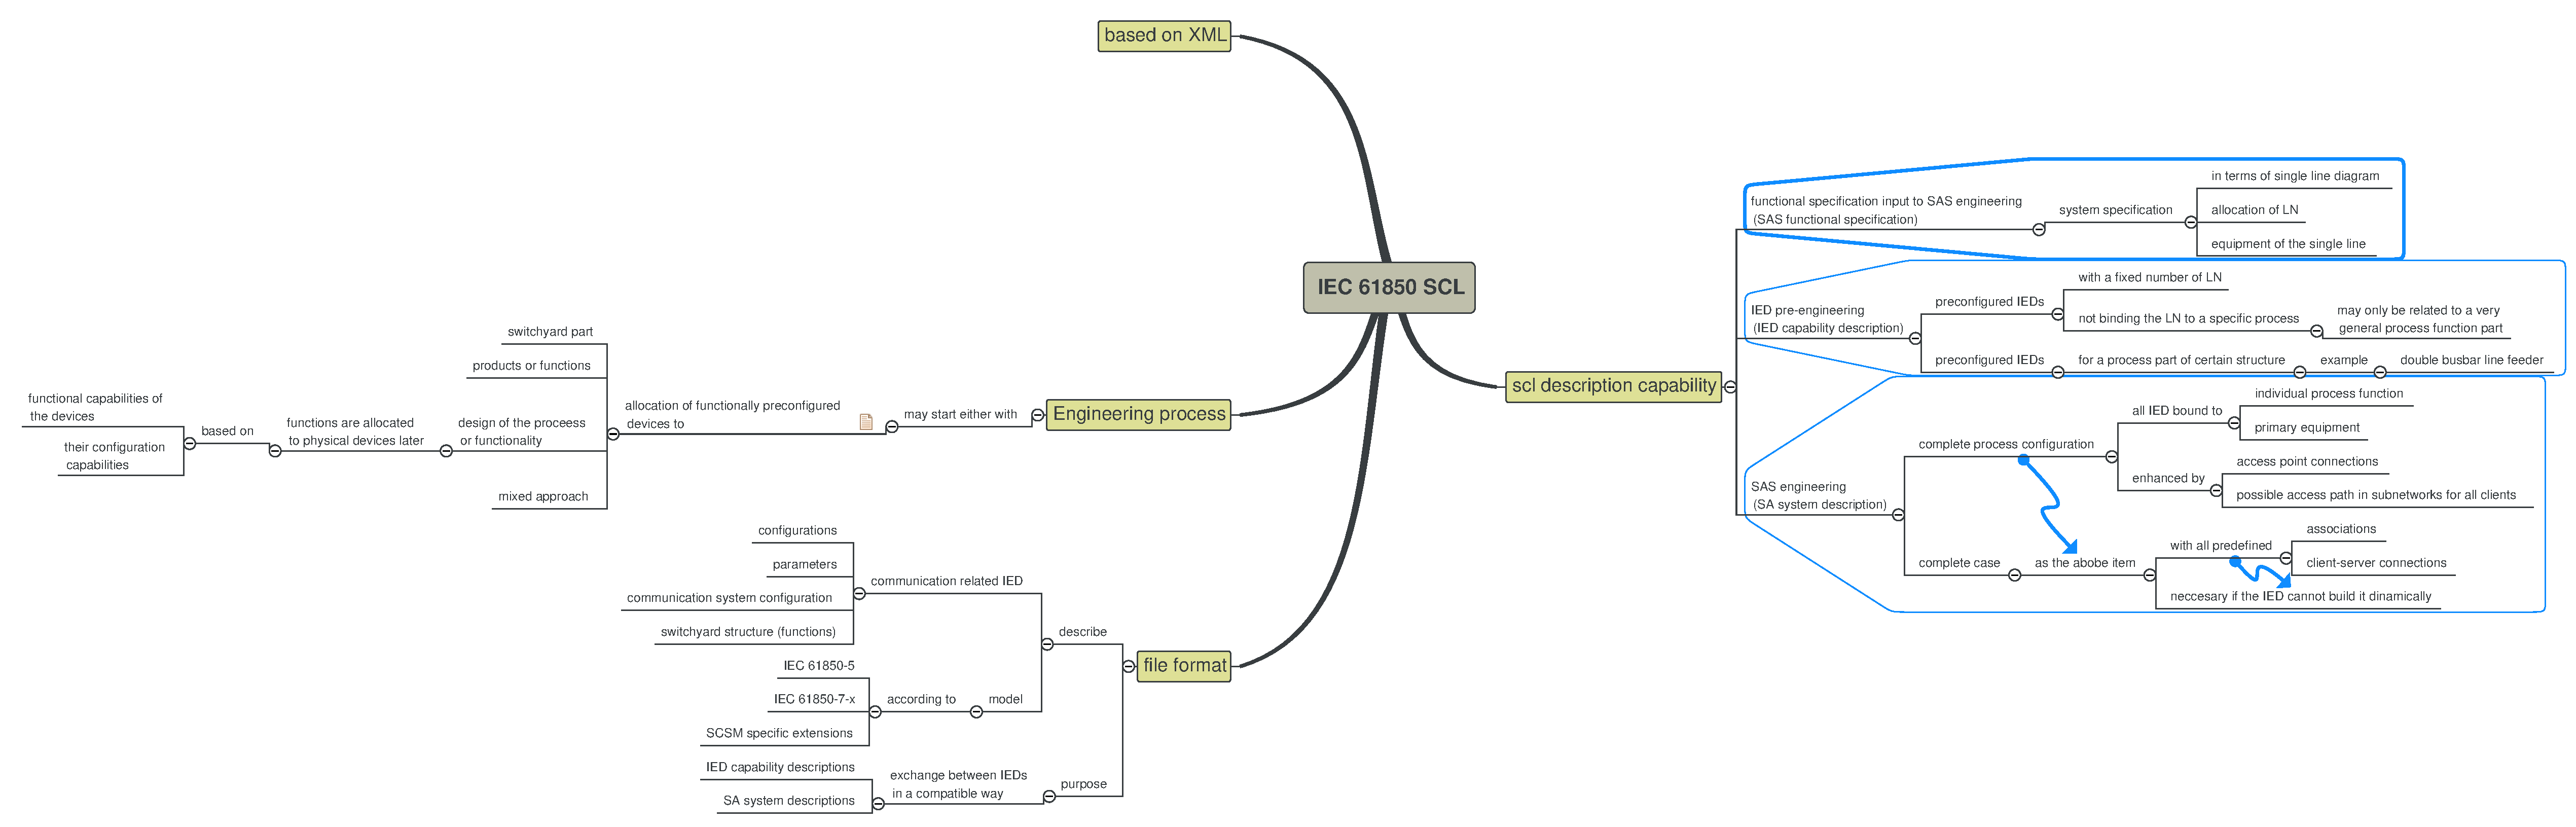
\includegraphics[width=1.0\textwidth]{appendices/IEC61850SCL}
%  \caption{Borrador - Esquema del futuro capitulo }
%  \label{fig:lan-networks-topologies-fig4}
%\end{figure}

\subsection{Variantes SCL}

Los archivos \gls{SCL}, dependiendo de su contenido, 
seg�n la IEC 61850--6 (Edici�n 1) \cite{IEC61850-6:2004} 
se clasifican en:

\begin{itemize}
  \item SSD: La variante SSD (\emph{System Specification Description}) 
  contiene el diagrama unifilar de la subestaci�n (a trav�s de los elementos
  \textbf{Header}, \textbf{Substation} y opcionalmente el elemento
  \textbf{DataTypeTemplates}).
  \item ICD: La variante ICD (\emph{IED Capability Description}) 
  describe las capacidades de los IEDs (IEDs a�n no configurados)
  (A trav�s de los elementos \textbf{IED}, \textbf{Communication},
  \textbf{Header} y \textbf{DataTypeTemplates}).
  \item CID: La variante CID (\emph{Configured IED Description}) 
  es la descripci�n de configuraci�n
  de un IED. Incluye todas las configuraciones IEC 61850 
  que puedan ser configurables: asociaciones, parametrizaciones
  de la red, entre otros.   (A trav�s de los elementos \textbf{IED}, 
  \textbf{Communication}, \textbf{Header} y \textbf{DataTypeTemplates}).
  A diferencia de la variante ICD, un CID tambi�n contiene 
  datos de los dem�s IEDs con los cuales se comunica.
  \item SCD: La variante SCD (\emph{Substation Configuration Description}) 
  contiene los archivos CID y su 
  relaci�n con respecto a la estructura del sistema el�ctrico
  descripto en el SSD, que tambi�n est� incluido en el SCD.
  (Contiene todos los elementos SCL, que pueden ser observados en 
  la figura \ref{fig:SCL-main-parts}.  
\end{itemize}
 
\section{Herramientas de ingenier�a}

Como apoyo fundamental para la ejecuci�n de estas tareas, la norma IEC 61850
contempla y define las llamadas herramientas de ingenier�a, que son programas
altamente especializados concebidos para elaborar los archivos necesarios para
especificar y configurar el sistema de automatizaci�n de una subestaci�n
el�ctrica que incorpore a la norma IEC 61850 como patr�n de comunicaciones [2].
Estas herramientas deber�an ofrecer una amplia gama de funcionalidades, como,
por ejemplo, la posibilidad de configurar dispositivos de marcas diferentes que
integren un mismo sistema, con base en las caracter�sticas de interoperabilidad
perseguidas por la norma \cite{PTI:SESEP2010}.


De acuerdo a esta norma, las herramientas de ingenier�a necesarias para los
proyectos realizados en conformidad con la misma deben posibilitar la creaci�n
y documentaci�n de los procesos de ingenier�a, tales como: gerenciamiento del
proyecto, parametrizaci�n de dispositivos y documentaci�n del sistema de
automatizaci�n de subestaciones por medio de la utilizaci�n del \gls{SCL}.         


\section{Partes de la norma IEC 61850}

La norma IEC 61850 consta de varias 
partes. En cada una de ellas se trata 
un aspecto espec�fico sobre 
las redes y sistemas de comunicaci�n 
de subestaciones, y por extensi�n, 
de hidroel�ctricas.  
A continuaci�n, se citan las 
partes de la norma IEC 61850 
y su estado de publicaci�n
en la fecha de realizaci�n de este trabajo:

\begin{itemize}
  \item IEC 61850--1:2003 	\cite{IEC61850-1:2003}:
	Introduction and overview (TR Ed1:2003--04).


  \item IEC 61850--2:2003		\cite{IEC61850-2:2003}: 
	Glossary (TS Ed1:2003--08).

	
  \item IEC 61850--3:2002		\cite{IEC61850-3:2002}:  
	General requirements(IS Ed1:2002--02).
  
  
  \item IEC 61850--4:2002		\cite{IEC61850-4:2002}: 
	System and project management  (IS Ed1:2002--01).
  
  
  \item IEC 61850--5:2003		\cite{IEC61850-5:2003}:  
	Communication requirements for 
	functions and device models  (IS Ed1:2003--07).
  
  
  \item IEC 61850--6:2004		\cite{IEC61850-6:2004}:   
	Configuration description language
	for communication in electrical
	substations related to IEDs  (IS Ed1:2004--03).
  
  
  \item IEC 61850--7--1:2003	\cite{IEC61850-7-1:2003}:  
	Basic communication structure -- Principles and models  (IS Ed1:2003--07).
  
  
  \item IEC 61850--7--2:2003	\cite{IEC61850-7-2:2003}:  
	Basic communication structure -- 
	Abstract communication service interface (ACSI)  (IS Ed1:2003--05).
	  
  
  \item IEC 61850--7--3:2003	\cite{IEC61850-7-3:2003}:  
	Basic communication structure -- Common data classes  (IS Ed1:2003--05).
  
  
  \item IEC 61850--7--4:2003	\cite{IEC61850-7-4:2003}:  
	Basic communication structure -- 
	Compatible logical node classes and data classes  (IS Ed1:2003--05).
  
  
  \item IEC 61850--7--410:2007	\cite{IEC61850-7-410:2007}:  
	Hydroelectric power plants -- 
	Communication for monitoring and control  (IS Ed1:2007--08).
  
  
  \item IEC 61850--7--420:2009	\cite{IEC61850-7-420:2009}:  
	Communications systems for distributed 
	energy resources (DER) -- Logical nodes  (IS Ed1:2009--03).
  
  
  \item IEC 61850--7--430 \cite{IEC61850-7-430:200-X}:  
	Communication system for distribution 
	feeder and network equipment  (57/954/NP).
  
  
  \item IEC 61850--7--5:2010	\cite{IEC61850-7-5:2010}:  
Basic communication structure --� 
Usage of information models for substation
automation applications  (DC 2010-08).
  
  
  \item IEC 61850--7--500:2010	\cite{IEC61850-7-500:2010}:  
	Use of logical nodes to model functions 
	of a substation automation system  (DC 2010--08).
  
  
  \item IEC 61850--7--510:2009	\cite{IEC61850-7-510:2009}:  
	Use of logical nodes to model 
	functions of a hydro power plant  (DC 2009--12).
  
  
  \item IEC 61850--7--520:2010	\cite{IEC61850-7-520:2010}:  
	Use of logical nodes to model functions 
	of distributed energy resources  (Draft 2010).
  
  
  \item IEC 61850--7--10:2009	\cite{IEC61850-7-10:2009}: 
	Web--based and structured access to the 
	IEC 61850 information models  (DC 2009--12).
  
  
  \item IEC 61850--8--1:2004	\cite{IEC61850-8-1:2004}: 
	Specific communication service 
	mapping (SCSM) -- 
	Mappings to MMS (ISO/IEC 9506--1 and 
	ISO/IEC 9506--2) and to ISO/IEC 8802--3  (IS Ed1:2004--05).
	  
  
  \item IEC 61850--9--1:2003	\cite{IEC61850-9-1:2003}:
	Specific communication service mapping (SCSM) -- 
	Sampled values over serial unidirectional
	multidrop point to point link  (IS Ed1:2003--05).
  
  
  \item IEC 61850--9--2:2004	\cite{IEC61850-9-2:2004}:
	Specific communication service mapping (SCSM) -- 
	Sampled values over ISO/IEC 8802--3  (IS Ed1:2004--04).

  
  \item IEC 61850--80--1 \cite{IEC61850-80-1:200-XXXXXX}:
	Guideline to exchanging information from a 
	CDC--based data model using IEC 60870--5--101 or IEC
	60870--5--104  (TS Ed1:2008--12).
  
  
  \item IEC 61850--90--1 \cite{IEC61850-90-1:200-XXXXXX}:
	Using IEC 61850 for the communication 
	between substations  (TS Ed1:2009--08).
  
  
  \item IEC 61850--90--2 \cite{IEC61850-90-2:200-XXXXXX}:
	Using IEC 61850 for the communication 
	between substations and control centres  (Draft 2010--01).
  
  
  \item IEC 61850--90--3 \cite{IEC61850-90-3:200-XXXXXX}:
	Using IEC 61850 for Condition Monitoring  (Draft 2010--06).
  
  
  \item IEC 61850--90--4 \cite{IEC61850-90-4:200-XXXXXX}:
	Network Engineering Guidelines  (Draft 2010--04).
  
  
  \item IEC 61850--90--5 \cite{IEC61850-90-5:200-XXXXXX}:
	Using IEC 61850 to transmit 
	synchrophasor information according to IEEE C37.118  (Draft 2010--06).
  
  
\end{itemize}
 
 
Cada parte de la norma est� compuesta por cl�usulas 
(en los Tissues \cite{IEC61850:tissues} se utiliza este nombre para las
secciones de cada parte de la norma), y nuevamente, 
cada cl�usula posee uno o m�s p�rrafos. En este trabajo,
al realizar las citaciones de esta norma, el autor 
referencia las cla�sulas (en caso que sea necesario) de la siguiente 
forma: \cite[cl. 1]{IEC61850-1:2003}.


\section{Partes de la norma IEC 61850 utilizadas para modelar la informaci�n de centrales hidro--el�ctricas}

De entre las partes mencionadas en la secci�n anterior destacamos las m�s importantes para este trabajo de modelado de la informaci�n 
del sistema de regulaci�n de una unidad generadora t�pica de Itaipu:

\begin{itemize}
  \item IEC 61850--7--4:2003	\cite{IEC61850-7-4:2003}:  
	Basic communication structure -- 
	Compatible logical node classes and data classes  (IS Ed1:2003--05).
  \item IEC 61850--7--410:2007	\cite{IEC61850-7-410:2007}:  
	Hydroelectric power plants -- 
	Communication for monitoring and control  (IS Ed1:2007--08).
\end{itemize}

La parte 7--4--10 define formalmente los nodos l�gicos para centrales hidroel�ctricas, mientras que la parte 7--4 
define los nodos l�gicos m�s generales, utilizados tanto en hidroel�ctricas, subestaciones, u otra �rea del sistema el�ctrico. 

Este apartado tiene relaci�n con la utilizaci�n de los nodos l�gicos en hidroel�ctricas, pero 
durante la realizaci�n de este trabajo este documento a�n se encontraba en proceso de redacci�n, 
y no se ha tenido acceso al borrador durante la elaboraci�n del presente trabajo.
\begin{itemize}
  \item  IEC 61850--7--510:2009	\cite{IEC61850-7-510:2009}:  
	Use of logical nodes to model 
	functions of a hydro power plant  (DC 2009--12).
\end{itemize}


\section{Descripci�n del regulador de velocidad actual de una unidad generadora t�pica de Itaipu}

Los generadores hidroel�ctricos de la Itaipu est�n interconectados a los sistemas el�ctricos del Paraguay y del Brasil. Uno 
de los requisitos m�s importantes para dicha interconexi�n es que los generadores deben estar sincronizados a la frecuencia 
del sistema. Para ello, los sistemas de regulaci�n de velocidad abren o cierran las paletas del distribuidor de la turbina para controlar su rotaci�n  
en funci�n a la carga, controlando asi la variaci�n de frecuencia hasta l�mites permitidos. El regulador de velocidad tambi�n 
controla la velocidad de rotaci�n sin carga de la unidad durante la fase de puesta en marcha, 
permitiendo una r�pida sincronizaci�n con el sistema. El papel del regulador puede extenderse 
a su participaci�n en la regulaci�n secundaria de un esquema de intercambio de cargas de potencia/frecuencia entre �reas.

Estos regualadores de velocidad se clasifican como reguladores electro-hidr�ulicos 
anal�gicos del tipo acelero-tacom�trico con estatismo y constan de circuitos hidr�ulicos encargados 
de mover las paletas del distribuidor (tanques, v�lvulas, servomotores), 
circuitos neum�ticos que acumulan energ�a potencial en forma de aire comprimido que poseen un 
transductor electro-hidr�ulico que sirve como interfaz de comando
y de circuitos electr�nicos que controlan el desv�o y la rapidez de variaci�n de la velocidad de rotaci�n de la unidad generadora 
a trav�s de una acci�n proporcional, integral y derivativa (PID). 

El documento \cite{Itaipu:195860C8841ER0} describe la estructura del regulador de velocidad de la siguiente manera:
\emph{``El regulador de velocidad `Rapid 77' posee una
estructura en dos niveles jer�rquicos, en la cual el sector
de la regulaci�n de velocidad y de carga se halla f�sica y
funcionalmente separado del sector de posicionamiento.
La realimentaci�n para el PID es tomada desde la se�al
el�ctrica suministrada a la v�lvula principal de distribuci�n
del aceite, y el circuito hidr�ulico de los servomotores,
que sirve para posicionar los �labes del distribuidor,
posee sus propios medios de realimentaci�n por v�a de
una se�al tomada de los transductores ubicados sobre
el mecanismo de operaci�n de los �labes y sobre el
husillo de la v�lvula principal de distribuci�n, v�ase la
figura \ref{fig:estructura-rv-rapid77}. Esta estructura en dos niveles facilita la
configuraci�n del regulador de velocidad, asiste al
mantenimiento y mejora la confiabilidad operacional.''}
La tabla \ref{table:esquema-funcional-rv} describe este esquema de la figura \ref{fig:estructura-rv-rapid77}.

\begin{figure}
\begin{center}
  \includegraphics[width=1.0\linewidth]{chapters/introduction/figures/estructura-rv-rapid77.eps}
  \caption{Estructura funcional del regulador Rapid 77}
  \label{fig:estructura-rv-rapid77}
\end{center}
\end{figure}


\subsection{Caracter�sticas b�sicas}

El sistema de regulaci�n actual est� constituido por tres circuitos: El circuito hidr�ulico, el circuito de aire comprimido,
y el circuito regulador electr�nico, cuyo esquema funcional es indicado en la figura \ref{fig:esquema-funcional-rv-rapid77}.

\subsubsection{El circuito regulador electr�nico}
B�sicamente, est� compuesto de:
\begin{itemize}
	\item Circuitos sensibles a la frecuencia del grupo
	\item Dispositivos de regulaci�n de carga -- frecuencia y retroalimentaciones de potencia y de apertura.
	\item Mezclador general y amplificador de potencia.
	\item Limitador de apertura o de potencia.
	\item Circuito posicionador y amplificador de potencia.
	\item Circuito taquim�trico auxiliar.
\end{itemize}

\subsubsection{El circuito hidr�ulico}
El principio de funcionamiento y su conjunci�n con el circuito el�ctrico se encuetra esquem�ticamente descripto en 
la figura \ref{fig:cadena-hidraulica-del-rv}. Sus componentes b�sicos son:


\begin{itemize}
	\item Transductor electro -- hidr�ulico (Actuador)
	\item V�lvula distribuidora
	\item Servomotor
	\item Tanques de aire/aceite
	\item Bombas de aceite
	\item V�lvula de aislamiento
	\item Sistema de amortiguamiento
	\item Sobrevelocidad hidromec�nica
	\item Tanque de aceite (tanque sin presi�n)
\end{itemize}


\subsubsection{El sistema de aire comprimido}
\begin{itemize}
	\item Grupo moto--compresores de alta presi�n (3 etapas).
	\item Tanque de aire comprimido
	\item Eletrov�lvula BE
\end{itemize}

\begin{figure}
\begin{center}
  \includegraphics[width=1.0\linewidth]{chapters/introduction/figures/cadena-hidraulica-del-rv.eps}
  \caption{Esquema funcional del conjunto electro-hidr�ulico del regulador}
  \label{fig:cadena-hidraulica-del-rv}
\end{center}
\end{figure}


\begin{figure}
\begin{center}
  \includegraphics[width=1.0\linewidth]{chapters/introduction/figures/esquema-funcional-rv-rapid77.eps}
  \caption{Esquema funcional del conjunto electro-hidr�ulico del regulador.}
  \label{fig:esquema-funcional-rv-rapid77}
\end{center}
\end{figure}



\begin{table}[H]
\begin{center}
\begin{tabular}{|p{0.7cm}|p{6.5cm}|p{0.8cm}|p{7.5cm}|}
	\cellcolor[gray]{0.8} \textbf{Nro.} & \cellcolor[gray]{0.8} \textbf{Descripci�n} & \cellcolor[gray]{0.8} \textbf{Nro.} & \cellcolor[gray]{0.8} \textbf{Descripci�n}\\
	\hline
	1 & Convertidor est�tico  & 24 & Actuador \\
	\hline
	2 & Repartidor de tensi�n & 25 & Polarizaci�n de marcha en vac�o \\
	\hline
	3 & Transformador de tensi�n del grupo & 26 & Vari�metro de retroceso del distribuidor \\
	\hline
	4 & Transformador de tensi�n de la red & 27 & Distribuidor hidr�ulico \\
	\hline
	5 & Cuarzo patr�n de frecuencia & 28 & Filtro de aceite \\
	\hline
	6 & Vari�metro de carga - frecuencia & 29 & Circuito hidr�ulico de regulaci�n \\
	\hline
	7 & Motoreductor & 30 & Detecci�n \\
	\hline
	8 & Detecci�n & 31 & Transductor vatim�trico \\
	\hline
	9 & Circuito frecuencim�trico & 32 & Potenci�metro de consigna del limitadorde abertura \\
	\hline
	10 & Regulaci�n del estatismo transitorio & 33 & Moto reductor \\
	\hline
	11 & Regulaci�n del Tr del estatismo transitorio & 34 & Servomotor \\
	\hline
	12 & Regulaci�n del Tv del aceler�metro & 35 & Leva \\
	\hline
	13 & Orden exterior & 36 & Vari�metro de retroceso del servomotor \\
	\hline
	14 & Regulaci�n del estatismo permanente & 37 & Turbina \\
	\hline
	15 & Primer mezclador & 38 & Alternador \\
	\hline
	16 & Programa & 39 & TC del alternador \\
	\hline
	17 & Teleregulaci�n & 40 & TP del alternador \\
	\hline
	18 & Orden exterior & R3 & Rel� de sincronizaci�n \\
	\hline
	19 & Mezclador general & R5 & Elecci�n de retroalimentaci�n de potencia o de abertura \\
	\hline
	20 & Comparador limitador & R7 & Programa o carga - frecuencia \\
	\hline
	21 & Circuito limitador & R10 & En reposo antes de acoplar \\
	\hline
	22 & Amplificador de potencia & R12 & Elecci�n entre limitador de abertura o de potencia \\
	\hline
	23 & Detecci�n  &  &  \\
	\hline
\end{tabular}
\caption{Descripci�n de �tems del esquema funcional del conjunto electro-hidr�ulico del regulador}
\label{table:esquema-funcional-rv}
\end{center}
\end{table}








